% Options for packages loaded elsewhere
\PassOptionsToPackage{unicode}{hyperref}
\PassOptionsToPackage{hyphens}{url}
%
\documentclass[
  11pt,
  a4paper,
]{article}
\usepackage{amsmath,amssymb}
\usepackage{lmodern}
\usepackage{iftex}
\ifPDFTeX
  \usepackage[T1]{fontenc}
  \usepackage[utf8]{inputenc}
  \usepackage{textcomp} % provide euro and other symbols
\else % if luatex or xetex
  \ifXeTeX
    \usepackage{zxjatype} 
    \usepackage[ipaex]{zxjafont}
    \setromanfont{Times New Roman}
  \fi
  \usepackage{unicode-math}
  \defaultfontfeatures{Scale=MatchLowercase}
  \defaultfontfeatures[\rmfamily]{Ligatures=TeX,Scale=1}
\fi
% Use upquote if available, for straight quotes in verbatim environments
\IfFileExists{upquote.sty}{\usepackage{upquote}}{}
\IfFileExists{microtype.sty}{% use microtype if available
  \usepackage[]{microtype}
  \UseMicrotypeSet[protrusion]{basicmath} % disable protrusion for tt fonts
}{}
\usepackage{xcolor}
\IfFileExists{xurl.sty}{\usepackage{xurl}}{} % add URL line breaks if available
\IfFileExists{bookmark.sty}{\usepackage{bookmark}}{\usepackage{hyperref}}
\hypersetup{
  pdftitle={Appendix ``Text-Based Nudges Promoting Rubella Antibody Testing and Vaccination: Evidence from Nationwide Online Field Experiment in Japan''},
  hidelinks,
  pdfcreator={LaTeX via pandoc}}
\urlstyle{same} % disable monospaced font for URLs
\usepackage[left=3cm,right=3cm,top=3cm,bottom=3cm]{geometry}

\usepackage{setspace}
\renewcommand{\baselinestretch}{1.5}
\usepackage{float}

\usepackage{longtable,booktabs,array}
\usepackage{threeparttable, threeparttablex, multirow}
\usepackage{calc} % for calculating minipage widths
% Correct order of tables after \paragraph or \subparagraph
\usepackage{etoolbox}
\makeatletter
\patchcmd\longtable{\par}{\if@noskipsec\mbox{}\fi\par}{}{}
\makeatother
% Allow footnotes in longtable head/foot
\IfFileExists{footnotehyper.sty}{\usepackage{footnotehyper}}{\usepackage{footnote}}
\makesavenoteenv{longtable}
\usepackage{graphicx}
\makeatletter
\def\maxwidth{\ifdim\Gin@nat@width>\linewidth\linewidth\else\Gin@nat@width\fi}
\def\maxheight{\ifdim\Gin@nat@height>\textheight\textheight\else\Gin@nat@height\fi}
\makeatother
% Scale images if necessary, so that they will not overflow the page
% margins by default, and it is still possible to overwrite the defaults
% using explicit options in \includegraphics[width, height, ...]{}
\setkeys{Gin}{width=\maxwidth,height=\maxheight,keepaspectratio}
% Set default figure placement to htbp
\makeatletter
\def\fps@figure{htbp}
\makeatother
\setlength{\emergencystretch}{3em} % prevent overfull lines
\providecommand{\tightlist}{%
  \setlength{\itemsep}{0pt}\setlength{\parskip}{0pt}}
\setcounter{secnumdepth}{5}


\usepackage{float}
\ifLuaTeX
  \usepackage{selnolig}  % disable illegal ligatures
\fi

\makeatletter
\def\@fnsymbol#1{\ensuremath{\ifcase#1\or \dagger\or \ddagger\or
   \mathsection\or \mathparagraph\or \|\or **\or \dagger\dagger
   \or \ddagger\ddagger \else\@ctrerr\fi}}
    \makeatother
\title{Appendix
``Text-Based Nudges Promoting Rubella Antibody Testing and Vaccination:
Evidence from Nationwide Online Field Experiment in Japan''  }

\date{2022/04/17}



\begin{document}
\begin{spacing}{1}
  \maketitle
\end{spacing}

{
\setcounter{tocdepth}{2}
\tableofcontents
}
\hypertarget{appendix-appendix}{%
\appendix}


\clearpage

\hypertarget{overview-of-online-survey-experiment}{%
\section{Overview of Online Survey Experiment}\label{overview-of-online-survey-experiment}}

\begin{figure}[t]
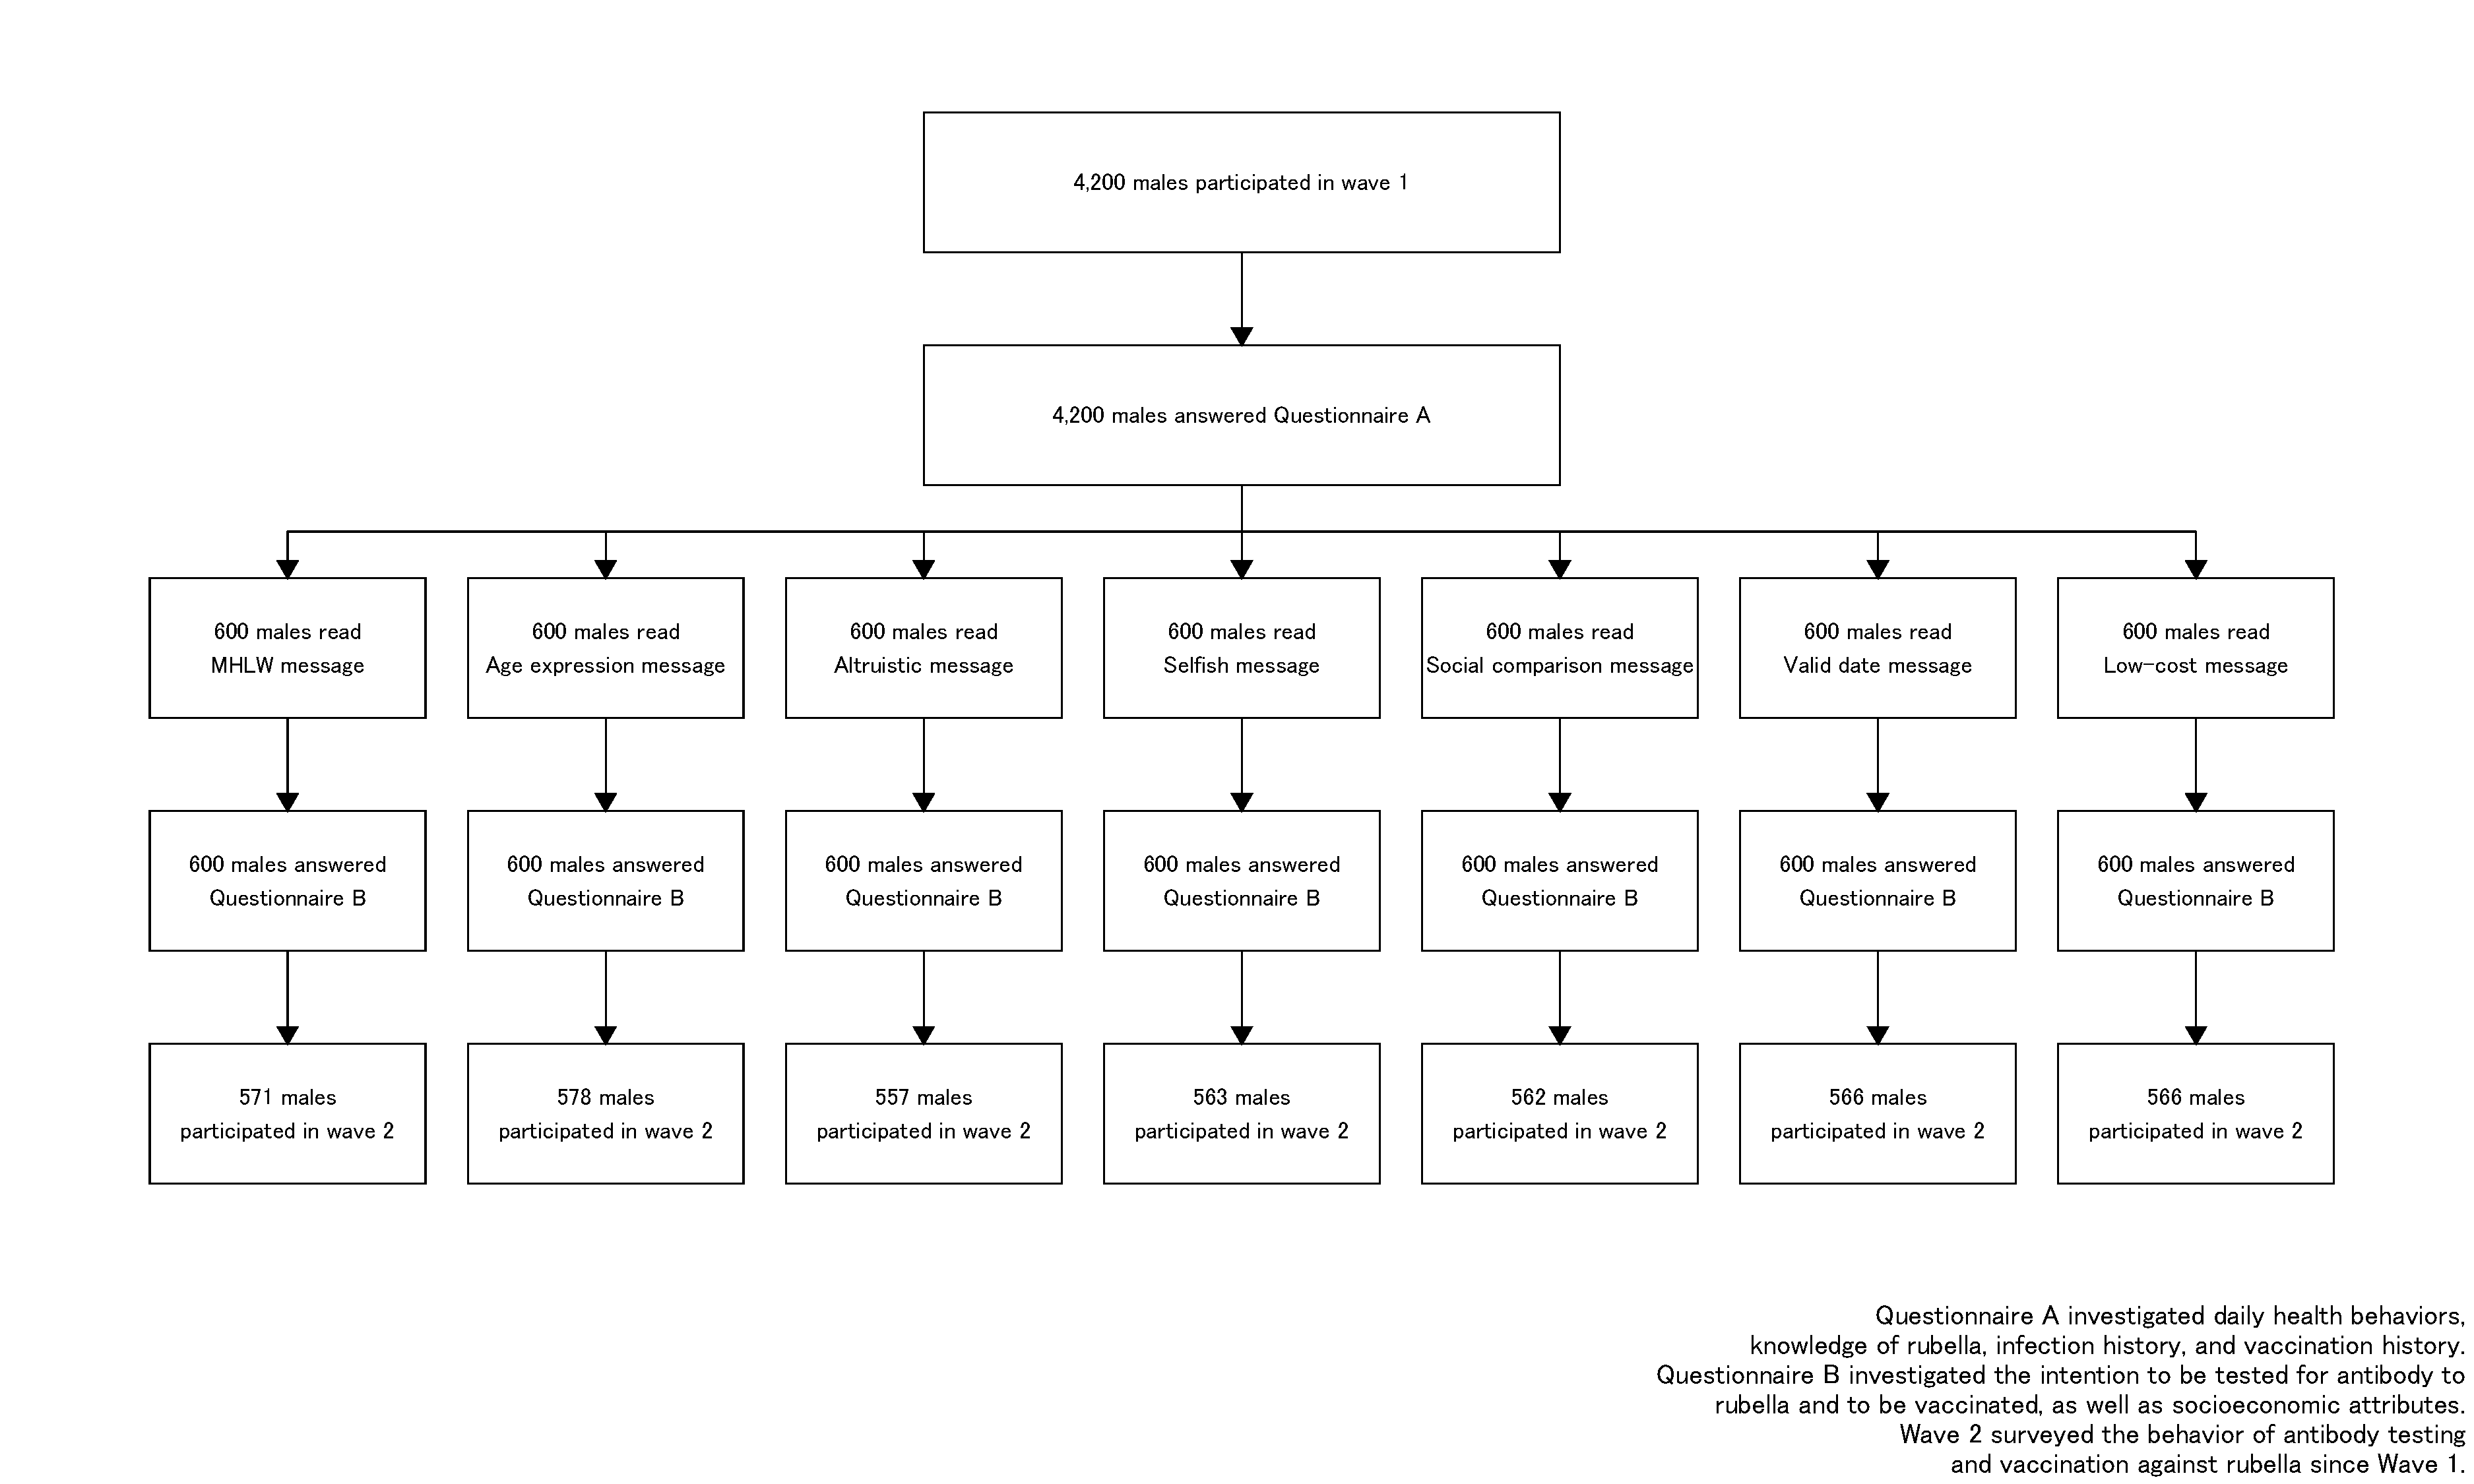
\includegraphics[width=1.5\linewidth,angle=90]{C:/Users/vge00/Desktop/2020-online-RCT/publish/appendix_files/figure-latex/flowchart-1} \caption{Overview of Online Survey Experiment}\label{fig:flowchart}
\end{figure}

\begin{table}[!h]

\caption{\label{tab:covlist}List of Covariates}
\centering
\fontsize{9}{11}\selectfont
\begin{tabular}[t]{l>{\raggedright\arraybackslash}p{30em}cc}
\toprule
  & Description & Mean & Std.Dev.\\
\midrule
age & (Wave1) Age as of April 2019 based on year of birth and month of birth. & 48.66 & 5.69\\
coupon2019 & (Wave1) Dummy variable taking one if 40 to 46 years old as of April 2019. & 0.35 & 0.48\\
married & (Wave1) Dummy variable taking one if a respondent is married. & 0.58 & 0.49\\
education & (Wave1) Years of education. & 14.75 & 2.31\\
exercise\_w1 & (Wave1) Dummy variable taking one if a respondent exercises or plays sports more than once a week. & 0.22 & 0.42\\
health\_check & (Wave1) Dummy variable taking one if a respondent has had medical examination at his/her city or place of employment in the past year from the time of the wave 1. & 0.68 & 0.46\\
flushot & (Wave1) Dummy variable taking one if a respondent is vaccinated against influenza every year. & 0.27 & 0.45\\
prob\_social & (Wave1) What percentage of men in their 40s and 50s does a respondent think may be infected with rubella? & 30.38 & 19.87\\
handicap & (Wave1) Dummy variable taking one if a respondent believes that if a woman in early pregnancy is infected with rubella, her child may be born with a disability. & 0.63 & 0.48\\
severity & (Wave1) Dummy variable taking one if a respondent believes that if an adult male is infected with rubella, it will become more severe. & 0.92 & 0.27\\
handwash & (Wave2) Five Likert scale for the question "I wash my hands and gargle frequently during the period from the end of the previous questionnaire response to today." & 3.91 & 1.04\\
temp\_check & (Wave2) Five Likert scale for the question "I take my tempature frequently during the period from the end of the previous questionnaire response to today." & 2.26 & 1.22\\
avoid\_out & (Wave2) Five Likert scale for the question "I am refraining from going out during the end of the previous questionnaire response to today." & 2.96 & 1.20\\
avoid\_crowd & (Wave2) Five Likert scale for the question "I avoid crowded places when I go out from the end of the previous questionnaire response to today." & 3.38 & 1.10\\
wear\_mask & (Wave2) Five Likert scale for the question "I always wear a medical mask when I go out or meet people during the period from the end of the previous questionnaire response to today." & 3.14 & 1.38\\
\bottomrule
\end{tabular}
\end{table}

\clearpage

\hypertarget{results-of-balance-test}{%
\section{Results of Balance Test}\label{results-of-balance-test}}

共変量のバランステストとして、各共変量の線形モデルを推定した。
このモデルの説明変数は介入群ダミーであり、厚労省メッセージ群を参照群とした。
我々は推定された線形モデルの係数すべてがゼロであるという帰無仮説をF検定によって検証した。
そのp値を表の最右列に示した。
表\ref{tab:int-coupon1-balance}は2019年度にクーポン券を自動的に受け取った人に限定した
wave 1 selection dataのバランステストの結果である。
表\ref{tab:int-coupon0-balance}は
2019年度にクーポン券を受け取るためにコストのかかる手続きが必要な人に限定した
wave 1 selection dataのバランステストの結果である。
表\ref{tab:act-coupon1-balance}は2019年度にクーポン券を自動的に受け取った人に限定した
wave 2 selection dataのバランステストの結果である。
表\ref{tab:act-coupon0-balance}は
2019年度にクーポン券を受け取るためにコストのかかる手続きが必要な人に限定した
wave 2 selection dataのバランステストの結果である。

\clearpage

\begin{table}[!h]

\caption{\label{tab:int-coupon1-balance}Balance Test of Wave 1 Selection Data (Men who automatically received coupon in 2019)}
\centering
\begin{tabular}[t]{l>{\centering\arraybackslash}p{3em}>{\centering\arraybackslash}p{3em}>{\centering\arraybackslash}p{3em}>{\centering\arraybackslash}p{3em}>{\centering\arraybackslash}p{3em}>{\centering\arraybackslash}p{3em}>{\centering\arraybackslash}p{3em}c}
\toprule
\multicolumn{1}{c}{ } & \multicolumn{7}{c}{Treatments} & \multicolumn{1}{c}{ } \\
\cmidrule(l{3pt}r{3pt}){2-8}
  & MHLW & Age expression & Altruistic & Selfish & Social comparison & Valid date & Low-cost & p-value\\
\midrule
age & 42.862 & 43.046 & 43.135 & 43.045 & 42.909 & 42.906 & 42.866 & 0.874\\
avoid\_crowd & 3.328 & 3.331 & 3.261 & 3.211 & 3.339 & 3.336 & 3.273 & 0.958\\
avoid\_out & 3.082 & 3.047 & 3.028 & 2.805 & 2.896 & 3.038 & 2.926 & 0.509\\
education & 14.654 & 14.473 & 14.595 & 14.205 & 14.099 & 14.348 & 14.575 & 0.446\\
exercise\_w1 & 0.246 & 0.176 & 0.277 & 0.189 & 0.165 & 0.217 & 0.213 & 0.285\\
flushot & 0.238 & 0.260 & 0.203 & 0.144 & 0.140 & 0.239 & 0.236 & 0.055\\
handicap & 0.638 & 0.550 & 0.595 & 0.568 & 0.537 & 0.543 & 0.520 & 0.502\\
handwash & 3.885 & 3.866 & 3.824 & 3.764 & 3.748 & 3.954 & 3.744 & 0.624\\
health\_check & 0.654 & 0.626 & 0.696 & 0.538 & 0.603 & 0.674 & 0.614 & 0.150\\
married & 0.408 & 0.458 & 0.412 & 0.417 & 0.455 & 0.478 & 0.480 & 0.785\\
prob\_social & 27.231 & 30.000 & 26.689 & 30.758 & 26.529 & 28.333 & 27.795 & 0.502\\
severity & 0.892 & 0.954 & 0.926 & 0.894 & 0.926 & 0.964 & 0.913 & 0.118\\
temp\_check & 2.180 & 2.260 & 2.380 & 2.179 & 2.226 & 2.145 & 2.157 & 0.735\\
wear\_mask & 2.951 & 3.063 & 3.113 & 3.033 & 2.965 & 3.115 & 3.174 & 0.852\\
\bottomrule
\end{tabular}
\end{table}
\begin{table}[!h]

\caption{\label{tab:int-coupon0-balance}Balance Test of Wave 1 Selection Data (Men who need to be processed to receive coupon in 2019)}
\centering
\begin{tabular}[t]{l>{\centering\arraybackslash}p{3em}>{\centering\arraybackslash}p{3em}>{\centering\arraybackslash}p{3em}>{\centering\arraybackslash}p{3em}>{\centering\arraybackslash}p{3em}>{\centering\arraybackslash}p{3em}>{\centering\arraybackslash}p{3em}c}
\toprule
\multicolumn{1}{c}{ } & \multicolumn{7}{c}{Treatments} & \multicolumn{1}{c}{ } \\
\cmidrule(l{3pt}r{3pt}){2-8}
  & MHLW & Age expression & Altruistic & Selfish & Social comparison & Valid date & Low-cost & p-value\\
\midrule
age & 51.632 & 51.408 & 51.226 & 51.657 & 51.582 & 51.545 & 51.502 & 0.712\\
avoid\_crowd & 3.307 & 3.378 & 3.429 & 3.250 & 3.306 & 3.296 & 3.455 & 0.354\\
avoid\_out & 2.903 & 2.917 & 2.919 & 2.884 & 2.825 & 2.966 & 2.982 & 0.848\\
education & 14.572 & 14.655 & 14.530 & 14.830 & 14.566 & 14.634 & 14.393 & 0.578\\
exercise\_w1 & 0.156 & 0.193 & 0.239 & 0.230 & 0.183 & 0.203 & 0.218 & 0.252\\
flushot & 0.228 & 0.244 & 0.197 & 0.270 & 0.275 & 0.228 & 0.251 & 0.433\\
handicap & 0.596 & 0.630 & 0.607 & 0.617 & 0.574 & 0.626 & 0.619 & 0.881\\
handwash & 3.803 & 3.883 & 3.900 & 3.778 & 3.817 & 3.833 & 3.892 & 0.827\\
health\_check & 0.632 & 0.664 & 0.701 & 0.683 & 0.653 & 0.659 & 0.644 & 0.742\\
married & 0.600 & 0.588 & 0.628 & 0.657 & 0.602 & 0.549 & 0.619 & 0.334\\
prob\_social & 26.920 & 31.387 & 30.983 & 28.522 & 29.442 & 27.846 & 31.925 & 0.025\\
severity & 0.920 & 0.933 & 0.919 & 0.970 & 0.940 & 0.931 & 0.908 & 0.046\\
temp\_check & 2.139 & 2.248 & 2.210 & 2.083 & 2.192 & 2.086 & 2.270 & 0.490\\
wear\_mask & 3.071 & 3.191 & 3.157 & 3.148 & 2.961 & 2.966 & 3.068 & 0.447\\
\bottomrule
\end{tabular}
\end{table}
\begin{table}[!h]

\caption{\label{tab:act-coupon1-balance}Balance Test of Wave 2 Selection Data (Men who automatically received coupon in 2019)}
\centering
\begin{tabular}[t]{l>{\centering\arraybackslash}p{3em}>{\centering\arraybackslash}p{3em}>{\centering\arraybackslash}p{3em}>{\centering\arraybackslash}p{3em}>{\centering\arraybackslash}p{3em}>{\centering\arraybackslash}p{3em}>{\centering\arraybackslash}p{3em}c}
\toprule
\multicolumn{1}{c}{ } & \multicolumn{7}{c}{Treatments} & \multicolumn{1}{c}{ } \\
\cmidrule(l{3pt}r{3pt}){2-8}
  & MHLW & Age expression & Altruistic & Selfish & Social comparison & Valid date & Low-cost & p-value\\
\midrule
age & 42.861 & 43.059 & 43.102 & 43.036 & 42.893 & 42.898 & 42.964 & 0.953\\
avoid\_crowd & 3.296 & 3.336 & 3.273 & 3.234 & 3.350 & 3.305 & 3.324 & 0.990\\
avoid\_out & 3.096 & 3.034 & 3.047 & 2.793 & 2.932 & 3.025 & 2.928 & 0.544\\
education & 14.496 & 14.471 & 14.547 & 14.126 & 14.010 & 14.407 & 14.595 & 0.474\\
exercise\_w1 & 0.252 & 0.185 & 0.266 & 0.171 & 0.165 & 0.195 & 0.225 & 0.375\\
flushot & 0.235 & 0.261 & 0.227 & 0.135 & 0.146 & 0.246 & 0.207 & 0.082\\
handicap & 0.652 & 0.563 & 0.602 & 0.568 & 0.544 & 0.542 & 0.514 & 0.425\\
handwash & 3.861 & 3.916 & 3.797 & 3.757 & 3.767 & 3.915 & 3.829 & 0.835\\
health\_check & 0.643 & 0.639 & 0.680 & 0.532 & 0.631 & 0.661 & 0.640 & 0.391\\
married & 0.391 & 0.454 & 0.391 & 0.360 & 0.437 & 0.466 & 0.477 & 0.467\\
prob\_social & 27.739 & 30.504 & 27.031 & 31.982 & 26.311 & 28.729 & 28.018 & 0.341\\
severity & 0.896 & 0.950 & 0.922 & 0.883 & 0.913 & 0.975 & 0.910 & 0.026\\
temp\_check & 2.139 & 2.235 & 2.414 & 2.126 & 2.204 & 2.203 & 2.117 & 0.535\\
wear\_mask & 2.930 & 3.076 & 3.109 & 3.009 & 3.010 & 3.144 & 3.207 & 0.794\\
\bottomrule
\end{tabular}
\end{table}
\begin{table}[!h]

\caption{\label{tab:act-coupon0-balance}Balance Test of Wave 2 Selection Data (Men who need to be processed to receive coupon in 2019)}
\centering
\begin{tabular}[t]{l>{\centering\arraybackslash}p{3em}>{\centering\arraybackslash}p{3em}>{\centering\arraybackslash}p{3em}>{\centering\arraybackslash}p{3em}>{\centering\arraybackslash}p{3em}>{\centering\arraybackslash}p{3em}>{\centering\arraybackslash}p{3em}c}
\toprule
\multicolumn{1}{c}{ } & \multicolumn{7}{c}{Treatments} & \multicolumn{1}{c}{ } \\
\cmidrule(l{3pt}r{3pt}){2-8}
  & MHLW & Age expression & Altruistic & Selfish & Social comparison & Valid date & Low-cost & p-value\\
\midrule
age & 51.695 & 51.394 & 51.179 & 51.662 & 51.421 & 51.605 & 51.512 & 0.564\\
avoid\_crowd & 3.295 & 3.361 & 3.447 & 3.239 & 3.313 & 3.309 & 3.433 & 0.437\\
avoid\_out & 2.886 & 2.889 & 2.932 & 2.866 & 2.855 & 2.964 & 2.941 & 0.960\\
education & 14.505 & 14.620 & 14.553 & 14.876 & 14.593 & 14.610 & 14.345 & 0.472\\
exercise\_w1 & 0.159 & 0.194 & 0.232 & 0.229 & 0.173 & 0.211 & 0.202 & 0.432\\
flushot & 0.223 & 0.245 & 0.189 & 0.264 & 0.280 & 0.215 & 0.241 & 0.376\\
handicap & 0.609 & 0.634 & 0.637 & 0.617 & 0.584 & 0.628 & 0.606 & 0.936\\
handwash & 3.823 & 3.889 & 3.926 & 3.751 & 3.836 & 3.861 & 3.867 & 0.769\\
health\_check & 0.632 & 0.667 & 0.684 & 0.677 & 0.645 & 0.673 & 0.631 & 0.849\\
married & 0.591 & 0.560 & 0.611 & 0.652 & 0.598 & 0.547 & 0.596 & 0.407\\
prob\_social & 27.409 & 31.296 & 30.368 & 29.055 & 30.187 & 28.072 & 32.118 & 0.130\\
severity & 0.923 & 0.935 & 0.926 & 0.970 & 0.935 & 0.933 & 0.921 & 0.171\\
temp\_check & 2.095 & 2.204 & 2.221 & 2.100 & 2.136 & 2.085 & 2.182 & 0.841\\
wear\_mask & 3.082 & 3.176 & 3.116 & 3.144 & 2.977 & 2.942 & 3.010 & 0.533\\
\bottomrule
\end{tabular}
\end{table}

\clearpage

\hypertarget{estimation-results-of-linear-probability-models}{%
\section{Estimation Results of Linear Probability Models}\label{estimation-results-of-linear-probability-models}}

\begin{table}

\caption{\label{tab:int-reg}Linear Probability Model of Intentions}
\centering
\begin{tabular}[t]{lcc}
\toprule
\multicolumn{1}{c}{ } & \multicolumn{1}{c}{Antibody Test} & \multicolumn{1}{c}{Vaccination} \\
\cmidrule(l{3pt}r{3pt}){2-2} \cmidrule(l{3pt}r{3pt}){3-3}
  & (1) & (2)\\
\midrule
Age expression & -0.036 & -0.099**\\
 & (0.038) & (0.043)\\
Altruistic & 0.051 & -0.059\\
 & (0.042) & (0.045)\\
Selfish & 0.026 & -0.052\\
 & (0.040) & \vphantom{1} (0.043)\\
Social comparison & -0.044 & -0.098**\\
 & (0.038) & (0.042)\\
Valid date & 0.028 & -0.044\\
 & (0.039) & (0.043)\\
Low-cost & 0.032 & -0.051\\
 & (0.040) & (0.043)\\
Coupon & -0.072 & -0.074\\
 & (0.052) & (0.062)\\
Coupon×Age expression & 0.045 & 0.103\\
 & (0.063) & (0.075)\\
Coupon×Altruistic & 0.089 & 0.073\\
 & (0.067) & (0.075)\\
Coupon×Selfish & 0.059 & 0.099\\
 & (0.066) & (0.075)\\
Coupon×Social comparison & 0.122* & 0.127*\\
 & (0.065) & \vphantom{1} (0.075)\\
Coupon×Valid date & -0.006 & 0.026\\
 & (0.064) & (0.074)\\
Coupon×Low-cost & 0.015 & 0.064\\
 & (0.065) & (0.075)\\
\midrule
Num.Obs. & 2459 & 2459\\
R2 & 0.363 & 0.530\\
R2 Adj. & 0.355 & 0.524\\
Covariates & X & X\\
\bottomrule
\end{tabular}
\end{table}
\begin{table}

\caption{\label{tab:int-reg-ftest}Effects of Text-Based Nudges on Intentions Using Linear Probability Model Estimates}
\centering
\begin{tabular}[t]{>{\raggedright\arraybackslash}p{5em}lcccccc}
\toprule
\multicolumn{2}{c}{ } & \multicolumn{3}{c}{Antibody Test} & \multicolumn{3}{c}{Vaccination} \\
\cmidrule(l{3pt}r{3pt}){3-5} \cmidrule(l{3pt}r{3pt}){6-8}
How to get coupons & Text-based nudges & estimate & std.error & p.value & estimate  & std.error  & p.value \\
\midrule
Costly procedure & Age expression & -0.036 & 0.038 & 0.336 & -0.099 & 0.043 & 0.021\\
 & Altruistic & 0.051 & 0.042 & 0.229 & -0.059 & 0.045 & 0.191\\
 & Selfish & 0.026 & 0.040 & 0.520 & -0.052 & 0.043 & 0.235\\
 & Social comparison & -0.044 & 0.038 & 0.247 & -0.098 & 0.042 & 0.020\\
 & Valid date & 0.028 & 0.039 & 0.482 & -0.044 & 0.043 & 0.308\\
 & Low-cost & 0.032 & 0.040 & 0.422 & -0.051 & 0.043 & 0.244\\
Automatic receiving & Age expression & 0.008 & 0.051 & 0.869 & 0.004 & 0.061 & 0.945\\
 & Altruistic & 0.140 & 0.052 & 0.007 & 0.014 & 0.060 & 0.810\\
 & Selfish & 0.085 & 0.052 & 0.101 & 0.048 & 0.061 & 0.435\\
 & Social comparison & 0.078 & 0.052 & 0.134 & 0.029 & 0.062 & 0.641\\
 & Valid date & 0.022 & 0.050 & 0.662 & -0.018 & 0.061 & 0.769\\
 & Low-cost & 0.048 & 0.051 & 0.345 & 0.014 & 0.062 & 0.826\\
\bottomrule
\end{tabular}
\end{table}
\begin{table}

\caption{\label{tab:int-reg-ftest2}Effects of Text-Based Nudges on Intentions Using Linear Probability Model Estimates (Baseline: Altruistic Message)}
\centering
\begin{tabular}[t]{>{\raggedright\arraybackslash}p{5em}lcccccc}
\toprule
\multicolumn{2}{c}{ } & \multicolumn{3}{c}{Antibody Test} & \multicolumn{3}{c}{Vaccination} \\
\cmidrule(l{3pt}r{3pt}){3-5} \cmidrule(l{3pt}r{3pt}){6-8}
How to get coupons & Text-based nudges & estimate & std.error & p.value & estimate  & std.error  & p.value \\
\midrule
Costly procedure & Age expression & -0.087 & 0.042 & 0.037 & -0.040 & 0.046 & 0.386\\
 & Selfish & -0.025 & 0.044 & 0.574 & 0.007 & 0.046 & 0.878\\
 & Social comparison & -0.095 & 0.042 & 0.024 & -0.039 & 0.045 & 0.388\\
 & Valid date & -0.023 & 0.043 & 0.591 & 0.015 & 0.046 & 0.739\\
 & Low-cost & -0.018 & 0.044 & 0.675 & 0.008 & 0.046 & 0.859\\
Automatic receiving & Age expression & -0.132 & 0.052 & 0.012 & -0.010 & 0.057 & 0.860\\
 & Selfish & -0.055 & 0.053 & 0.303 & 0.033 & 0.058 & 0.560\\
 & Social comparison & -0.062 & 0.054 & 0.248 & 0.014 & 0.058 & 0.804\\
 & Valid date & -0.118 & 0.052 & 0.022 & -0.032 & 0.057 & 0.572\\
 & Low-cost & -0.092 & 0.052 & 0.077 & -0.001 & 0.058 & 0.988\\
\bottomrule
\end{tabular}
\end{table}

クーポン券が自動的に送付されるかどうかは年齢で決まるので、
サブサンプルを用いたナッジ・メッセージの効果は
クーポン券が自動的に送付されるかどうかだけでなく、
二つのサブサンプルの年齢の違いの影響を受けている。
この問題を排除するために、我々は以下のような意向の線形確率モデルを推定した。
\begin{align}
  Y_{ij} = \alpha + \sum_j \beta_j \text{Message}_j
           + \sum_j \gamma_j (\text{Message}_j \times \text{Coupon}_i)
           + \delta \text{Coupon}_i + \lambda X'_{ij} + \epsilon_{ij},
\end{align}
ここで、\(\text{Message}_j\)は厚労省メッセージ群をコントロールとした介入群ダミーであり、
\(\text{Coupon}_i\)はクーポン券の自動送付を受け取ったことを示すダミー変数である。
\(X\)は個人の共変量ベクトルであり、年齢を含む。

関心のあるパラメータは\(\beta_j\)と\(\gamma_j\)である。
クーポンを自動的に受け取れる男性に限定した
ナッジ・メッセージ\(j\)の効果は\(\hat{\beta}_j\)である。
一方で、
クーポン券を受け取るためにはコストのかかる手続きが必要な男性に限定した
ナッジ・メッセージ\(j\)の効果は\(\hat{\beta}_j + \hat{\gamma}_j\)である。

表\ref{tab:int-reg}は線形確率モデルの結果である。また、
表\ref{tab:int-reg-ftest}は
線形確率モデルの推定値を用いたナッジ・メッセージの効果である。
本論で示したt検定の結果と同様に、
2019年度にクーポン券が自動的に送付される男性における
利他強調メッセージの抗体検査の意向に対する効果は統計的に有意であるが、
2019年度にクーポン券を取得するために手続きが必要な男性における
利他強調メッセージの抗体検査の意向に対する効果は統計的に非有意である。
さらに、表\ref{tab:int-reg}より、この二つの効果の差は統計的に非有意である。

また、本論で示したt検定の結果と同様に、
2019年度にクーポン券が自動的に送付される男性における
社会比較メッセージのワクチン接種の意向に対する効果は統計的に非有意であるが、
2019年度にクーポン券を取得するために手続きが必要な男性における
社会比較メッセージのワクチン接種の意向に対する効果は統計的に有意に負である。
その効果は-9.8\%ポイントであり、二群の平均値の差より大きい。
さらに、表\ref{tab:int-reg}より、
この二つの効果の差は統計的に10\%水準で有意である。

2019年度にクーポン券を取得するために手続きが必要な男性における
年齢表現メッセージのワクチン接種の意向に対する効果は-9.9\%ポイントであり、
統計的に5\%水準で有意である。
t検定で推定された効果の規模は-6.6\%ポイントであり、
共変量の有無で効果の規模が大きく異なる。

表\ref{tab:int-reg-ftest2}は利他強調メッセージをコントロールとした
他のナッジ・メッセージの効果の推定結果である。
2019年度にクーポン券を受け取るためにはコストのかかる手続きが必要な男性における
ナッジ・メッセージの効果の差は\(\beta_j - \beta_{\text{Altruistic}}\)
で得られる。
2019年度にクーポン券を自動的に受け取った男性における
ナッジ・メッセージの効果の差は\((\beta_j + \gamma_j) - (\beta_{\text{Altruistic}} + \gamma_{\text{Altruistic}})\)
で得られる。
2019年度にクーポン券が自動的に送付される男性に限定したとき、
利己強調メッセージ・社会比較メッセージの抗体検査の意向は
利他強調メッセージのそれと統計的に有意に異ならない。
この意味で、利己強調メッセージや社会比較メッセージは
抗体検査の意向を促進している可能性がある。
しかしながら、検出力を十分に保てるほどの差ではないので、
サンプルサイズを大きくして再度検証すべきである。

\begin{table}

\caption{\label{tab:act-reg}Linear Probability Model of Behaviors}
\centering
\begin{tabular}[t]{lcc}
\toprule
\multicolumn{1}{c}{ } & \multicolumn{1}{c}{Antibody Test} & \multicolumn{1}{c}{Vaccination} \\
\cmidrule(l{3pt}r{3pt}){2-2} \cmidrule(l{3pt}r{3pt}){3-3}
  & (1) & (2)\\
\midrule
Age expression & 0.003 & 0.004\\
 & (0.008) & (0.005)\\
Altruistic & 0.016 & 0.005\\
 & (0.011) & (0.005)\\
Selfish & 0.008 & 0.005\\
 & (0.010) & (0.005)\\
Social comparison & 0.021* & -0.001\\
 & (0.012) & (0.001)\\
Valid date & 0.009 & 0.005\\
 & (0.009) & (0.005)\\
Low-cost & 0.005 & -0.001\\
 & (0.008) & (0.001)\\
Coupon & 0.017 & 0.001\\
 & (0.020) & (0.011)\\
Coupon×Age expression & 0.029 & 0.004\\
 & (0.029) & (0.015)\\
Coupon×Altruistic & 0.057* & 0.033\\
 & (0.034) & (0.022)\\
Coupon×Selfish & 0.054 & 0.014\\
 & (0.033) & (0.019)\\
Coupon×Social comparison & 0.036 & 0.041*\\
 & (0.035) & (0.023)\\
Coupon×Valid date & -0.002 & -0.005\\
 & (0.026) & (0.013)\\
Coupon×Low-cost & 0.033 & 0.020\\
 & (0.031) & (0.018)\\
\midrule
Num.Obs. & 2272 & 2272\\
R2 & 0.077 & 0.037\\
R2 Adj. & 0.066 & 0.025\\
Covariates & X & X\\
\bottomrule
\end{tabular}
\end{table}
\begin{table}

\caption{\label{tab:act-reg-ftest}Effects of Text-Based Nudges on Behaviors Using Linear Probability Model Estimates}
\centering
\begin{tabular}[t]{>{\raggedright\arraybackslash}p{5em}lcccccc}
\toprule
\multicolumn{2}{c}{ } & \multicolumn{3}{c}{Antibody Test} & \multicolumn{3}{c}{Vaccination} \\
\cmidrule(l{3pt}r{3pt}){3-5} \cmidrule(l{3pt}r{3pt}){6-8}
How to get coupons & Text-based nudges & estimate & std.error & p.value & estimate  & std.error  & p.value \\
\midrule
Costly procedure & Age expression & 0.003 & 0.008 & 0.724 & 0.004 & 0.005 & 0.413\\
 & Altruistic & 0.016 & 0.011 & 0.152 & 0.005 & 0.005 & 0.405\\
 & Selfish & 0.008 & 0.010 & 0.448 & 0.005 & 0.005 & 0.324\\
 & Social comparison & 0.021 & 0.012 & 0.084 & -0.001 & 0.001 & 0.538\\
 & Valid date & 0.009 & 0.009 & 0.339 & 0.005 & 0.005 & 0.317\\
 & Low-cost & 0.005 & 0.008 & 0.520 & -0.001 & 0.001 & 0.610\\
Automatic receiving & Age expression & 0.032 & 0.028 & 0.259 & 0.008 & 0.014 & 0.592\\
 & Altruistic & 0.073 & 0.032 & 0.023 & 0.038 & 0.021 & 0.071\\
 & Selfish & 0.061 & 0.032 & 0.054 & 0.019 & 0.017 & 0.267\\
 & Social comparison & 0.057 & 0.032 & 0.077 & 0.040 & 0.023 & 0.078\\
 & Valid date & 0.007 & 0.025 & 0.775 & 0.000 & 0.012 & 0.991\\
 & Low-cost & 0.038 & 0.029 & 0.193 & 0.019 & 0.018 & 0.279\\
\bottomrule
\end{tabular}
\end{table}
\begin{table}

\caption{\label{tab:act-reg-ftest2}Effects of Text-Based Nudges on Behaviors Using Linear Probability Model Estimates (Baseline: Altruistic Message)}
\centering
\begin{tabular}[t]{>{\raggedright\arraybackslash}p{5em}lcccccc}
\toprule
\multicolumn{2}{c}{ } & \multicolumn{3}{c}{Antibody Test} & \multicolumn{3}{c}{Vaccination} \\
\cmidrule(l{3pt}r{3pt}){3-5} \cmidrule(l{3pt}r{3pt}){6-8}
How to get coupons & Text-based nudges & estimate & std.error & p.value & estimate  & std.error  & p.value \\
\midrule
Costly procedure & Age expression & -0.013 & 0.012 & 0.279 & -0.001 & 0.007 & 0.930\\
 & Selfish & -0.009 & 0.013 & 0.518 & 0.001 & 0.007 & 0.930\\
 & Social comparison & 0.005 & 0.015 & 0.740 & -0.005 & 0.005 & 0.345\\
 & Valid date & -0.008 & 0.013 & 0.556 & 0.000 & 0.007 & 0.989\\
 & Low-cost & -0.011 & 0.012 & 0.389 & -0.005 & 0.005 & 0.347\\
Automatic receiving & Age expression & -0.041 & 0.036 & 0.247 & -0.030 & 0.022 & 0.177\\
 & Selfish & -0.012 & 0.038 & 0.755 & -0.018 & 0.024 & 0.447\\
 & Social comparison & -0.016 & 0.039 & 0.686 & 0.003 & 0.028 & 0.917\\
 & Valid date & -0.066 & 0.033 & 0.046 & -0.038 & 0.020 & 0.066\\
 & Low-cost & -0.035 & 0.036 & 0.341 & -0.019 & 0.024 & 0.443\\
\bottomrule
\end{tabular}
\end{table}

意向の線形確率モデルと同じように、
我々は行動を被説明変数とした線形確率モデルを推定した。
表\ref{tab:act-reg}は線形確率モデルの結果である。また、
表\ref{tab:act-reg-ftest}は線形確率モデルの推定値を用いた
ナッジ・メッセージの効果である。
その結果、二群の平均値の差の推定と同様の結果を得られた。
それに加えて、2019年度にクーポン券が自動的に送付される男性における
社会比較メッセージの抗体検査の受検率に対する効果は5.7\%ポイントで、
統計的に10\%水準で有意である。
また、表\ref{tab:act-reg}より、
利他強調メッセージの抗体検査受検率に対する効果と
社会比較メッセージのワクチン接種率に対する効果は
クーポン券の受け取り方によって異なり、
これは統計的に10\%水準で有意である。

表\ref{tab:act-reg-ftest2}は利他強調メッセージを参照群とした
メッセージの効果の推定結果である。
利他強調メッセージ以外のナッジ・メッセージの抗体検査受検率は
利他強調メッセージのそれと有意に異ならない。
この意味で、他のナッジ・メッセージも抗体検査の受検を促進しているかもしれないが、
検出力を十分に保てるほどの差でない。

\clearpage

\end{document}
